\section{Kapitel 10}
\subsection{Aufgabenstellung}
Wir sollen ein Programm schreiben Welches ein Artikel von der Tagesschau herunterlädt und
anschlie\ss end in einer Datei abspeichert. Der Nutzer kann angeben, welche Datei er einlesen möchte,
anschlie\ss end kann er die gezählten Wörter in Alphabetischer Reihenfolge ausgeben lassen.
Zusätzlich soll über ein Startparameter entschieden werden, ob Gro\ss -  und Kleinschreibung
beachtet wird.

\subsection{Anforderungsdefinition}
\begin{enumerate}
	\item Ein Artikel der Tagesschau mit mehr als 500 Wörtern soll runter geladen werden.
	\item Die Wörter sollen in einer geeigneten Collection abgelegt werden,
	\item Die Wörter sollen Sortiert ausgegeben können.
	\item Bei der Ausgabe der Wörte wird zusätzlich die Häufigkeit mit angegeben.
	\item Beim Start soll entschieden werden ob Gro\ss - oder Kleinschreibung.
\end{enumerate}

\subsection{Entwurf}
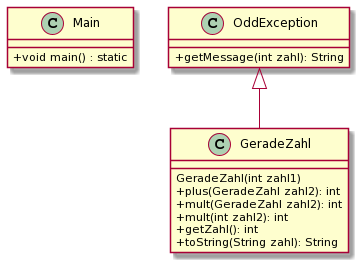
\includegraphics[scale=0.55]{uml/uml_c8_p1.png}

\subsection{Quelltext}
\subsubsection{Main.java}
\lstinputlisting[language = Java , frame = trBL , escapeinside={(*@}{@*)}]{../chapter_10/src/chapter_10/Main.java}
\subsubsection{IO.java}
\lstinputlisting[language = Java , frame = trBL , escapeinside={(*@}{@*)}]{../chapter_10/src/chapter_10/IO.java}
\subsubsection{MyException.java}
\lstinputlisting[language = Java , frame = trBL , escapeinside={(*@}{@*)}]{../chapter_10/src/chapter_10/MyException.java}

\subsection{Testdokumentation}
\begin{itemize}
	\item Startparameter:
	\subitem Bei einem inkorrekten Startparameter wird eine Exception geworfen.
	\item Menüauswahl:
	\subitem Bei falscher Eingabe wurde eine entsprechende Fehlermeldung ausgegeben.
	\item Artikel herunterladen:
	\subitem Wenn der Link nicht existiert kommt eine Fehlermeldung.
	\item Datei Laden:
	\subitem Wenn keine Datei gefunden wird mit den Namen kommt eine Fehlermeldung.
	\item Wörter ausgeben:
	\subitem Wenn keine Datei geladen wurde, kommt eine entsprechende Fehlermeldung.
\end{itemize}

\subsection{Benutzungshinweise}
Bei dem Aufruf des Programmes muss mit true oder false angegeben werden, ob Gro\ss - und
Kleinschreibung zu beachten ist. Anschlie\ss end kann man in dem Menü auswählen ob man einen
Artikel von der Tagesschau herunterladen möchte, eine Datei einlesen oder die Wörter in 
Alphabetischer Reihenfolge ausgibt.

\subsection{Anwendungsbeispiel}
\begin{lstlisting}[frame = trBL , escapeinside={(*@}{@*)}]
	[sebastian@laptop bin]$ java Main 	
	Exception in thread "main" chapter_10.MyException: Error, nur true oder false erlaubt
	at chapter_10.Main.main(Main.java:21)
	[sebastian@laptop bin]$ 
	[sebastian@laptop bin]$ java Main 
	Bitte wähle einer der Folgenden Optionen aus:
	1) Einen Artikel von der Tagesschau herunterladen.
	2) Eine Datei laden.
	3) Wörter ausgeben.
	0) Programm Beenden.
	1
	Bitte gebe den Link an:
	lasdfl
	Loading Content
	Es konnte keine Verbindung hergestellt werden. Bitte überprüfen Sie die angegebene address, oder ihre Internetverbindung!
	Error, kein Inhalt gefunden!
	
	Bitte wähle einer der Folgenden Optionen aus:
	1) Einen Artikel von der Tagesschau herunterladen.
	2) Eine Datei laden.
	3) Wörter ausgeben.
	0) Programm Beenden.
	1
	Bitte gebe den Link an:
	https://www.tagesschau.de/inland/bundeslaender-schulen-corona-101.html
	Loading Content
	Loading done
	Data written do file called: Bei Schulen gehen die Länder Sonderwege.txt
	
	Bitte wähle einer der Folgenden Optionen aus:
	1) Einen Artikel von der Tagesschau herunterladen.
	2) Eine Datei laden.
	3) Wörter ausgeben.
	0) Programm Beenden.
	2
	Bitte geben Sie den Dateinamen an:
	Test
	Error, es wurde noch keine Datei geladen!
	
	Bitte wähle einer der Folgenden Optionen aus:
	1) Einen Artikel von der Tagesschau herunterladen.
	2) Eine Datei laden.
	3) Wörter ausgeben.
	0) Programm Beenden.
	3
	Es wurde noch keine Datei Geladen!
	
	Bitte wähle einer der Folgenden Optionen aus:
	1) Einen Artikel von der Tagesschau herunterladen.
	2) Eine Datei laden.
	3) Wörter ausgeben.
	0) Programm Beenden.
	2
	Bitte geben Sie den Dateinamen an:
	Bei Schulen gehen die Länder Sonderwege
	Datei wurde Erfolgreich geladen
	
	Bitte wähle einer der Folgenden Optionen aus:
	1) Einen Artikel von der Tagesschau herunterladen.
	2) Eine Datei laden.
	3) Wörter ausgeben.
	0) Programm Beenden.
	3
	ab 6x
	aber 1x
	Abitur 1x
	Abschlussklassen 4x
	Abschlussprüfungen 1x
	Abständen 1x
	abzumelden 1x
	aktiv 1x
	alle 2x
	allen 1x
	als 2x
	also 1x
	alten 1x
	am 1x
	an 6x
	andere 1x
	anderen 1x
	anders 2x
	Anfang 1x
	angeboten 1x
	Anmeldequote 1x
	anschließend 1x
	Anschluss 1x
	anzubieten 1x
	Appelle 1x
	Auch 1x
	auch 5x
	auf 5x
	aufgehoben 1x
	aus 2x
	ausgesetzt 2x
	Ausnahmen 1x
	ausnehme 1x
	Baden-Württembergsgrüner 1x
	Bayernlässt 1x
	bedeute 1x
	begrüßte 1x
	Bei 3x
	bei 1x
	beide 1x
	beim 1x
	bekommen 1x
	berechtigt 1x
	beschlossen 1x
	beschlossene 1x
	Beschlusses 1x
	Beschlüsse 1x
	beschränkt 1x
	besonders 2x
	besser 1x
	bestehende 1x
	betonte 1x
	betreffe 1x
	Betreuung 1x
	Betreuungsmöglichkeit 1x
	betroffene 1x
	Bildung 1x
	bis 4x
	bisher 2x
	bisherigen 1x
	bislang 1x
	bisschen 1x
	bleibe 1x
	bleibt 1x
	Blick 1x
	Brandenburg 1x
	Britta 1x
	Bund 2x
	Bund-Länder-Beratungen 1x
	Bund-Länder-Beschlüsse 1x
	Bund-Länder-Beschlüssen 1x
	Bund-Länder-Treffen 1x
	Bundes 1x
	Bundesländer 1x
	CDU 1x
	Chance 1x
	Christian 1x
	Corona-Pandemie 1x
	Corona-Schutz-Verordnung 1x
	CSU 1x
	da 1x
	Dabei 1x
	dabei 1x
	daher 1x
	damit 1x
	dann 1x
	Das 3x
	das 3x
	dass 4x
	dem 5x
	demnach 1x
	Den 1x
	den 5x
	denen 1x
	dennoch 1x
	Der 2x
	der 18x
	Deren 1x
	des 3x
	desto 1x
	deutlich 2x
	Die 6x
	die 19x
	Dienstag 1x
	Dienstagabend 1x
	Dies 2x
	dies 2x
	diese 1x
	Distanzunterricht 1x
	Dresden 1x
	Dreyer 1x
	eben 1x
	ebenfalls 2x
	eher 1x
	eigene 1x
	eigentlich 2x
	Ein 1x
	ein 2x
	Eine 1x
	eine 4x
	einem 1x
	einen 3x
	einer 1x
	Einfluss 1x
	eingeschränkt 1x
	eingeschränkten 2x
	einiger 1x
	einmalig 1x
	einschränkte 1x
	einzelne 1x
	Eltern 4x
	Entscheidung 1x
	Entscheidungen 1x
	entschied 1x
	entsprechenden 1x
	Er 3x
	er 1x
	erfolgen 1x
	erhalten 1x
	erklärte 1x
	erläuterten 1x
	Ermahnungen 1x
	Ernst 1x
	erste 2x
	erweiterte 1x
	Es 2x
	es 6x
	fast 1x
	Februar 8x
	Fernunterricht 1x
	fest 1x
	folgen 1x
	Formblatt 1x
	fortgesetzt 1x
	Fragen 1x
	fünften 1x
	Für 1x
	für 11x
	gar 1x
	geben 1x
	gebeten 1x
	gebracht 1x
	gehen 4x
	geht 1x
	gehört 1x
	genug 1x
	geplant 1x
	gerade 1x
	gesamte 1x
	geteilten 1x
	gibt 1x
	Grant 1x
	Grundschulen 3x
	Grundschüler 2x
	Grundschülern 1x
	grundsätzlich 2x
	haben 3x
	Hamburgverschärft 1x
	hart 1x
	hatten 1x
	Hause 1x
	Hendrik 1x
	hier 2x
	hoffe 1x
	hohe 1x
	hänge 1x
	Höhe 1x
	ihre 4x
	im 9x
	immer 1x
	In 1x
	in 16x
	Infektionsgeschehen 2x
	Infektionslage 1x
	Infektionszahlen 1x
	Inzidenzwert 1x
	inzwischen 1x
	ist 2x
	Jahrgänge 1x
	Januar 1x
	je 2x
	jedoch 2x
	Jugendlichen 1x
	Kabinettssitzung 2x
	Kanzlerin 1x
	Kaum 1x
	Kein 1x
	keine 2x
	Kern 1x
	Kind 1x
	Kinder 4x
	Kitas 10x
	Klasse 2x
	Klassen 1x
	Klassenstufen 1x
	kleinen 1x
	KMK 1x
	kommenden 1x
	Konkret 1x
	Kretschmann 1x
	Kritikerin 1x
	Kultusminister 2x
	Kultusministerkonferenz 1x
	Kurs 1x
	können 1x
	kündigte 1x
	lassen 1x
	liegen 1x
	Lockdowns 1x
	Länder 6x
	Ländern 1x
	Ländersache 1x
	machte 1x
	MainzIn 1x
	Malu 1x
	manche 1x
	Manuela 1x
	Markus 1x
	Maßnahme 1x
	Maßnahmen 1x
	Mecklenburg-Vorpommern 1x
	Mecklenburg-Vorpommerns 1x
	Merkel 1x
	Ministerpräsident 2x
	Ministerpräsidenten 1x
	Ministerpräsidentin 2x
	Ministerpräsidentinnen 1x
	mit 5x
	möglich 1x
	Möglichkeit 1x
	mühsam 1x
	München 1x
	nach 4x
	NDR 1x
	neuen 1x
	nicht 5x
	Niedersachsen 1x
	Niedersachsenbefreit 1x
	noch 4x
	Notbetreuung 1x
	Notfall 1x
	nur 6x
	oder 2x
	offen 1x
	per 1x
	Piwarz 1x
	planen 1x
	Pläne 1x
	positioniert 1x
	Präsenzpflicht 4x
	Präsenzunterricht 6x
	pädagogische 1x
	rechtfertigen 1x
	reduziert 1x
	Regelbetreuung 1x
	Regelbetrieb 1x
	Regeln 2x
	Regelung 1x
	Regelungen 1x
	Regierungschef 1x
	restriktive 2x
	restriktiven 1x
	Rheinland-Pfalz 1x
	Routine 1x
	Runde 1x
	Sachsenhält 1x
	sagte 3x
	schicken 1x
	schon 1x
	schrittweise 1x
	schränkte 1x
	Schulbetrieb 1x
	Schulen 15x
	Schulschließung 1x
	Schwesig 2x
	Schüler 5x
	Schülern 1x
	sehr 1x
	sei 4x
	seien 1x
	sein 1x
	seine 1x
	seiner 1x
	Senat 1x
	sich 3x
	sie 1x
	siebten 1x
	sind 3x
	Situation 1x
	so 3x
	soll 5x
	solle 1x
	sollen 2x
	Sollten 1x
	sollten 4x
	Sonderwege 1x
	sorgfältig 1x
	SPD 3x
	SPD-Politikerin 1x
	später 1x
	stark 1x
	statt 1x
	stattfinden 1x
	steigen 1x
	Stephan 1x
	Söder 1x
	tageweise 1x
	Teil 1x
	Tisch 1x
	Tonne 2x
	trotz 1x
	tue 1x
	umsetzen 1x
	Umsetzung 2x
	Und 1x
	und 18x
	unter 1x
	Unterricht 1x
	unterrichtet 1x
	unterschiedlich 1x
	unterstrich 1x
	Unterstützung 1x
	vehemente 1x
	vereinbart 1x
	verkünden 1x
	verlängerten 1x
	verlängerter 1x
	verschärft 1x
	veränderbar 1x
	Viele 1x
	vom 5x
	Von 1x
	von 6x
	vorgehen 1x
	vorsichtig 1x
	Vorsitzende 1x
	vorzubereiten 1x
	war 1x
	warum 1x
	Wechsel 1x
	Wechselunterricht 3x
	Wege 1x
	Weil 1x
	weil 1x
	weiter 2x
	Weitere 1x
	weitere 1x
	weiterhin 2x
	weniger 1x
	Wenn 1x
	wenn 2x
	Wer 1x
	werde 1x
	werden 9x
	wie 1x
	wieder 4x
	Winfried 1x
	wir 1x
	wird 1x
	Woche 1x
	wollen 1x
	wonach 1x
	wurde 1x
	Zahl 1x
	Zahlen 1x
	zeigte 1x
	Zeit 1x
	zu 5x
	zugehen 1x
	zulasse 1x
	zulässt 1x
	zum 4x
	zumindest 1x
	zur 1x
	zurück 1x
	öffnen 2x
	Öffnungsschritte 1x
	Bitte wähle einer der Folgenden Optionen aus:
	1) Einen Artikel von der Tagesschau herunterladen.
	2) Eine Datei laden.
	3) Wörter ausgeben.
	0) Programm Beenden.
	0
	[sebastian@laptop bin]$ 
\end{lstlisting}